\chapter{Tinjauan Pustaka}

Pada bab ini berisi hasil tinjauan pustaka yang menjadi dasar analisis dan perancangan pada BAB III. Bab ini secara garis besar berupa teori keamanan perbatasan jaringan, tinjauan pustaka mengenai permasalahan yang dihadapi, solusi teoretis, dan tinjauan pustaka yang berkaitan dengan perancangan solusi. Solusi teoretis berupa klasifikasi deteksi intrusi, yakni \textit{anomaly-based} dan \textit{signature-based}.

\section{\textit{Network Border Security}}

Seperti dalam dunia nyata, sebuah keamanan dijaga pada sebuah wilayah tertentu. Pada sebuah jaringan \textit{border-security} memisahkan jaringan \textit{internal} dan \textit{external}. Jaringan \textit{internal} sebagai yang akan dilindungi, dan memisahkannya dengan \textit{external network} menggunakan sebuah \textit{gateway border}. Pada (Strebe, 2004) \textit{border-security} secara teori harus memiliki \textit{measures} sebagai berikut:

\begin{enumerate}
	\item \textit{Control every crossing}
	
	\textit{Border security} harus melakukan pengecekan untuk setiap lalu lintas data antara \textit{internal network} dan \textit{external network}. Sebuah koneksi antara \textit{internal network} dan \textit{external network} yang tidak dilakukan pengecekan
	dapat menjadi celah untuk terjadinya serangan. Hal ini dapat dilakukan dengan cara menempatkan firewall pada setiap batas jaringan.
	
	\item \textit{Apply the same policy universally}
	
	Sebuah \textit{control} untuk lalu lintas data tertentu harus dilakukan sama untuk seluruh hubungan yang terjadi antara \textit{internal network} dan \textit{external network}. Hal ini membutuhkan penerapan menyeluruh, karena efek dari penerapan ini akan bergantung pada penerapan yang terlemah. Jika dibutuhkan perbedaan tingkat keamanan, bisa dilakukan dengan memisahkan jaringan yang memerlukan perbedaan tingkat. Salah satunya seperti yang dilakukan pada DMZ.
	
	\item \textit{Deny by default}
	
	Seluruh keterhubungan hanya akan memperbolehkan lalu lintas data yang ada pada \textit{whitelist}. Penerapan ini perlu dilakukan untuk lalu lintas ke luar	maupun ke dalam firewall. Jika sebaliknya diterapkan \textit{allow by default}, ketika malware dengan jenis trojan tanpa sengaja dijalankan pada jaringan internal, malware dapat dengan mudah melakukan koneksi ke luar. Misal untuk mengirimkan data yang seharusnya dilindungi.
	
	\item \textit{Hide as much as information as possible}
	
	Penyembunyian data interior dari sebuah jaringan perlu dilakukan. Hal ini digunakan untuk mencegah penyerang mendapatkan informasi jaringan internal. Mendapatkan informasi mengenai jaringan internal merupakan langkah awal yang dilakukan \textit{hacker}. Jika informasi ini didapatkan, \textit{hacker} dapat menggunakan untuk berbagai macam, seperti \textit{inserting-traffic at IDS} (\cite{marpaung2012survey}).
	
\end{enumerate}

\section{Firewall}
Firewall merupakan perangkat keras, perangkat lunak atau kombinasi keduanya yang digunakan untuk melakukan pengawasan dan filter terhadap lalu lintas data yang masuk atau keluar dari sebuah jaringan yang berusaha dilindungi (\cite{kizza2002computer}). Menurut (Stallings, 2012) \textit{design goal firewall} sebagai berikut: 
Seluruh lalu lintas data dari dalam ke luar atau pun sebaliknya harus melalui firewall;
Hanya lalu lintas data yang terotorisasi yang dapat melalui firewall;
dan firewall merupakan sistem yang kebal terhadap \textit{penetration}.

Kekuatan dan kelemahan dari firewall menurut (Peterson, 2012):
Firewall dapat di-\textit{deploy} \textit{unilaterally};
Firewall tidak dapat membatasi akses antara host yang berada dalam \textit{internal-network};
Jika pihak diberikan akses ke internal-network, maka pihak tersebut menjadi \textit{security vulnerability};
Dan bug pada firewall yang dapat diakses dari \textit{internal-network} dapat menjadi masalah serius.

Firewall saat ini yang pada umumnya memiliki tipe sebagai berikut:

\begin{enumerate}
	\item \textit{Packet filtering firewall}
	\textit{Packet filtering firewall}
	
	Merupakan firewall yang menggunakan informasi dari protokol IP untuk menentukan apakah dilakukan teruskan atau buang untuk lalu lintas data masuk maupun keluar.
	
	\item \textit{Application proxy firewall}
	
	\textit{Application proxy firewall} atau \textit{application gateway} merupakan firewall yang digunakan pada \textit{application layer} untuk sebuah protocol tertentu.
\end{enumerate}

\section{Arsitektur Firewall}
Firewall pada implementasinya dapat ditempatkan dengan beberapa arsitektur menurut (\cite{zwicky2000building}).

\subsection{Arsitektur \textit{Dual-Homed Host}}

Arsitektur \textit{dual-homed host} merupakan dibangun dengan menggunakan komputer \textit{dual-homed host}, yakni sebuah komputer yang terhubung dengan dua atau lebih jaringan. Komputer ini dapat bekerja sebagai \textit{router} antara kedua jaringan yang terhubung ke komputer tersebut. Namun, untuk mengimplemntasi firewall dengan arsitektur \textit{dual-homed host} fungsi \textit{routing} ini tidak difungsikan. Sehingga tidak ada data yang dapat dikirimkan langsung antar kedua jaringan. Jadi untuk setiap paket yang akan dikirimkan dari jaringan internal ke jaringan luar harus melalui \textit{dual-homed host}, dan dari jaringan luar ke jaringan dalam juga harus melalui \textit{dual-homed host}. Sehingga susunan komponen pada jaringan tersebut seperti pada gambar \ref{fig:dual_homed}

\begin{figure}[H]
	\centering
	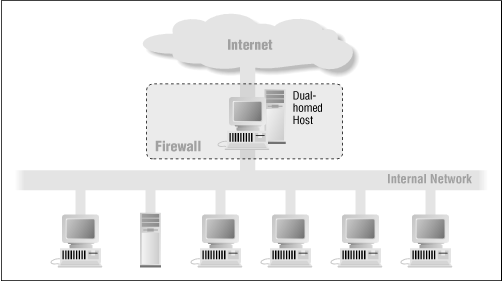
\includegraphics[width=300px]{resources/dual_homed.png}
	\caption{Arsitektur \textit{Dual-Homed}}
	\label{fig:dual_homed}
\end{figure}

\subsection{Arsitektur \textit{Screened Host}}

Berbeda dengan arsitektur \textit{dual-homed host} yang memberikan servis dari host yang terhubung ke beberapa jaringan dengan fungsi tidak mengaktifkan fungsi \textit{routing}, arsitektur \textit{screened host} memberikan layanan dari host yang hanya terhubung ke \textit{internal network} dan menggunakan \textit{router} terpisah seperti pada  gambar \ref{fig:screened_host}. Pada arsitektur ini, keamanan dijaga oleh \textit{packet filtering}, dengan melakukan konfigurasi berikut:

\begin{enumerate}
\item Memperbolehkan \textit{internal host} untuk dapat mengakses beberapa servis langsung tanpa melalui \textit{proxy}.
\item Melarang semua paket dari internal host. (Untuk memaksa host itu menggunakan \textit{proxy}).
\end{enumerate}

Namun pada pada arsitektur ini, jaringan internal sangat mudah diserang dari host \textit{bastion} yang berada pada \textit{internal network}. Sehingga bastion host menjadi sasaran yang paling diinginkan oleh penyerang. Karena tidak ada pertahanan lagi diantara internal host dan host lain yang berada pada jaringan internal.

\begin{figure}[H]
	\centering
	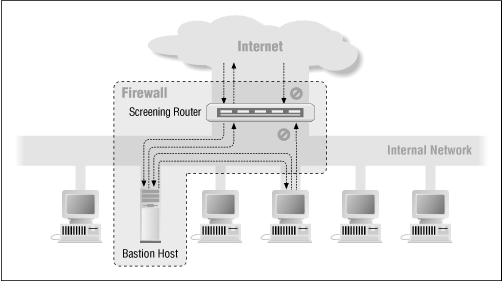
\includegraphics[width=300px]{resources/screened_host.png}
	\caption{Arsitektur \textit{Screened Host}}
	\label{fig:screened_host}
\end{figure}

\subsection{Arsitektur \textit{Screened Subnet}}

Arsitektur \textit{screened subnet} memiliki layer tambahan dibandingkan dengan arsitektur \textit{screened host} dengan memisahkan \textit{internal network} lebih jauh dari internet.

Arsitektur ini ditujukan agar host \textit{bastion}, yakni host yang dieskpos ke internet, merupakan host yang paling rentan untuk diserang. Meskipun host sudah dilakukan usaha untuk melindungi host tersebut, namun host tersebut menjadi titik paling jelas untuk diserang.

\begin{figure}[H]
	\centering
	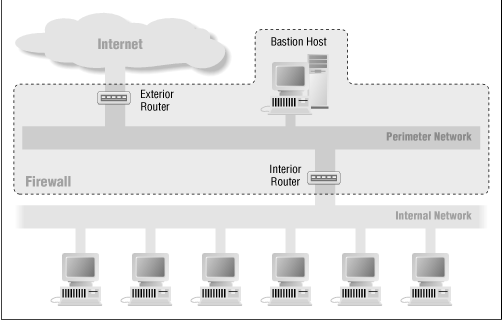
\includegraphics[width=300px]{resources/screened_subnet.png}
	\caption{Arsitektur \textit{Screened Subnet}}
	\label{fig:screened_subnet}
\end{figure}

\section{Next Generation Firewall}
Pada masa ini, firewall terbagi menjadi 2 yaitu tradisional firewall dan \textit{new generation firewall}. Hal ini terjadi karena tradisional firewall tidak lagi mumpuni untuk menahan serangan yang ada di dunia internet ini. 
Tradisional firewall adalah firewall yang bekerja di \textit{network layer}(\cite{nicoll2004challenges}), menggunakan port dan protokol IP untuk mengontrol dan mencegah serangan dari jaringan.(\cite{zhong2012design}) Skema dari tradisional firewall ini dapat dilihat pada gambar berikut.
\begin{figure}[H]
	\centering
	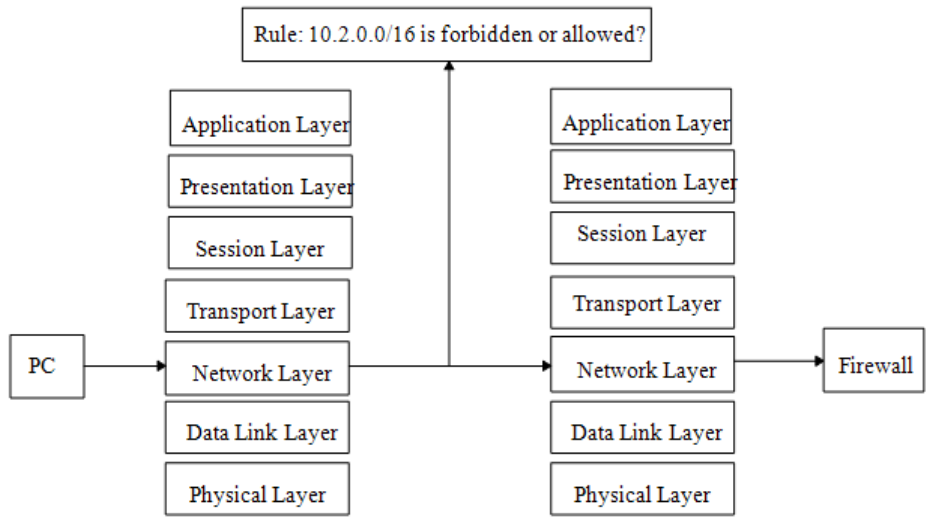
\includegraphics[width=0.8\textwidth]{resources/tradisional_firewall.png}
	\caption{Skema tradisional firewall(\cite{zhong2012design})}
	\label{fig:tradisional_firewall}
\end{figure}

Firewall ini hanya mengecek \textit{header} paket sesuai dengan port-nya, sehingga tidak dapat mengontrol aplikasi. Tradisional firewall yang memakai \textit{deep packet inspection} (DPI) untuk menambah keamanan juga tidak terlalu berhasil, karena memunculkan limitasi dan masalah baru. Menurut (\cite{miller2011next}), masalah tersebut adalah
\begin{itemize}
	\item Aplikasi yang tidak seharusnya berada di jaringan diperbolehkan masuk ke jaringan.
	\item Tidak semua paket yang harus diperiksa terperiksa
	\item \textit{Policy management} menjadi rumit dan berbelit
	\item Kinerja yang tidak memadai 
\end{itemize}

Sementara itu, \textit{Next Generation Firewall} (NGFW) merupakan pengembangan dari \textit{first-generation firewall} yang memiliki \textit{Deep Packet Inspection} (DPI). Secara fungsionalitas NGFW merupakan gabungan dari \textit{Intrusion Prevention System} (IPS) dan \textit{first-generation firewall}. NGFW dapat dipandang sebagai IPS karena NGFW memiliki \textit{awareness} terhadap \textit{application level payload}. Hasil pengecekan kemudian digunakan untuk memutuskan apakah paket di-forward atau di-drop. (Pescatore, 2009). \textit{New Generation Firewall} adalah firewall yang berjalan di atas layer aplikasi, untuk mendeteksi apakah paket tersebut sesuai dengan \textit{user`s rule} atau tidak(\cite{zhong2012design}). Skema dari \textit{new generation firewall} adalah sebagai berikut.
\begin{figure}[H]
	\centering
	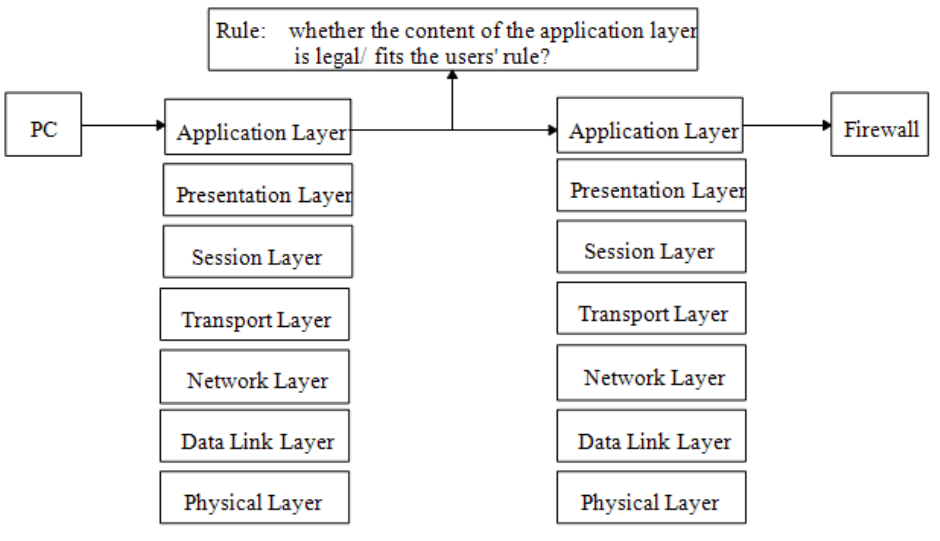
\includegraphics[width=\textwidth]{resources/NGFW.png}
	\caption{Skema new generation firewall(\cite{zhong2012design})}
	\label{fig:new_generation_firewall}
\end{figure}

Oleh karena itu, fungsi dan kemampuan utama yang dibutuhkan oleh \textit{new generation firewall} adalah:
\begin{itemize}
	\item Identifikasi aplikasi (port, protokol, \textit{evasive techniques}, atau \textit{SSL encryption}) sebelum melakukan hal apapun
	\item Menyediakan \textit{policy-based control} yang lebih jelas dan \textit{granular}
	\item Secara akurat mengidentifikasi pengguna dan menggunakan informasi tersebut sebagai atribut dari \textit{policy control}
	\item Menyediakan proteksi secara \textit{real-time} terhadap ancaman dari jaringan, termasuk yang beroperasi pada layer aplikasi.
	\item Terintegrasi untuk meningkatkan kapasitas pencegahan ancaman
\end{itemize}

Identifikasi yang digunakan pada NGFW adalah \textit{application identification}, \textit{user identification}, dan \textit{content identification}. \textit{Application identification} akan mengidentifikasi suatu aplikasi melalui port dan protokolnya, \textit{signatures} dan perilaku dari aplikasi tersebut. \textit{User identification} bertugas untuk mengidentifikasi pengguna jaringan. Sementara \textit{content identification} akan mengidentifikasi melalui isi data yang dibawa oleh lalu lintas data tersebut. \\

\noindent\textbf{Application identification}\\
Karena NGFW berjalan pada level aplikasi, maka pengenalan aplikasi adalah langkah awal yang sangat penting. Salah satu cara yang dipakai oleh \textit{traditional firewall} adalah pengenalan port dan protokolnya, namun teknik tersebut tidaklah lagi cukup. Maka, teknik Identifikasi aplikasi yang digunakan oleh \textit{new generation firewall} adalah 
\begin{itemize}
	\item Deteksi dan deskripsi aplikasi protokol\\
	Untuk mendeteksi protokol aplikasi sehingga dapat dianalisis lebih lanjut. Contohnya pada suatu HTTP, apakah menggunakan SSL atau tidak, sehingga lalu lintas data dapat dianalisis lebih jauh. 
	\item \textit{Decode} protokol aplikasi\\
	Untuk mendeteksi apakah protokol tersebut benar-benar digunakan oleh aplikasi yang semestinya, atau  ada aplikasi lain yang berjalan melalui protokol tersebut (tunnel). Contohnya seperti \textit{Yahoo! Instant Messenger} yang mungkin berada di dalam protokol HTTP.
	\item \textit{Application signatures}\\
	Untuk mengecek apakah aplikasi tersebut menggunakan port dan protokol
	yang sesuai dengan fungsinya. Identifikasi ini mengecek melalui \textit{attribute} atau karakteristik unik pada kontennya. Identifikasi ini juga mempunyai kemampuan untuk mengidentifikasi fungsi-fungsi spesifik didalam aplikasi, seperti transfer file.
	\item Heuristics\\
	Pada lalu lintas data yang menghindari identifikasi melalui analisis \textit{signature}, maka analisis \textit{heuristik} yang akan dilakukan oleh NGFW. Contoh dari penggunaan identifikasi ini adalah pada aplikasi P2P atau VoIP yang menggunakan enkripsi khusus pada aplikasinya. 
\end{itemize}

\noindent\textbf{User identification}\\
Teknologi ini memanfaatkan alamat IP untuk mengidentifikasi pengguna, untuk mengatur \textit{visibilitas} dan kontrol suatu aktivitas pada jaringan. Teknologi ini dapat digunakan untuk:
\begin{itemize}
	\item Mendapatkan \textit{visibilitas} tentang siapa yang bertanggung jawab untuk semua aplikasi, konten, dan ancaman lalu lintas data pada jaringan tersebut
	\item Mengizinkan penggunaan identitas sebagai variabel dalam \textit{access control policies}.
	\item Memfasilitasi \textit{troubleshooting/incident response}
\end{itemize}

\noindent\textbf{Content identification}\\
Teknologi ini membuat \textit{next generation firewall} dapat mencegah ancaman secara \textit{real-time}, mengontrol aktifitas \textit{browsing}, dan menyaring file atau data. Komponen dari teknologi ini adalah:
\begin{itemize}
	\item Pencegahan ancaman\\
	Komponen ini berfungsi untuk mencegah \textit{spyware}, virus, dan ancaman lainnya dari jaringan. Komponen ini dibantu oleh \textit{application decoder}, \textit{stream-based virus detection}, \textit{spyware scanning}, \textit{uniform threat signature format}, dan IPS.
	\item URL filtering\\
	Komponen ini menyaring konten melalui URL. Memiliki basis data berisikan URL yang terintegrasi membuat para administrator dapat memonitor dan mengatur aktivitas pengguna jaringan tersebut. 
	\item Filter file dan data\\
	Komponen ini menggunakan kelebihan dari \textit{in-depth application inspection} untuk mengurangi pengiriman file dan data yang tidak ter-otorisasi. Kelebihan ini juga termasuk dengan memblokir file sesuai tipe file yang sebenarnya, tidak hanya melihat \textit{extension}-nya, dan juga untuk mengatur pengiriman data-data yang sensitif seperti nomor kartu kredit. 
\end{itemize}

Pada tradisional firewall, fungsi-fungsi keamanan dilakukan secara terpisah satu sama lain, seperti yang digambarkan pada gambar \ref{fig:architecture_tradisional_firewall}. Hal ini menyebabkan penggunaan \textit{system resource} yang berlebihan dan tidak efisien.
\begin{figure}[H]
	\centering
	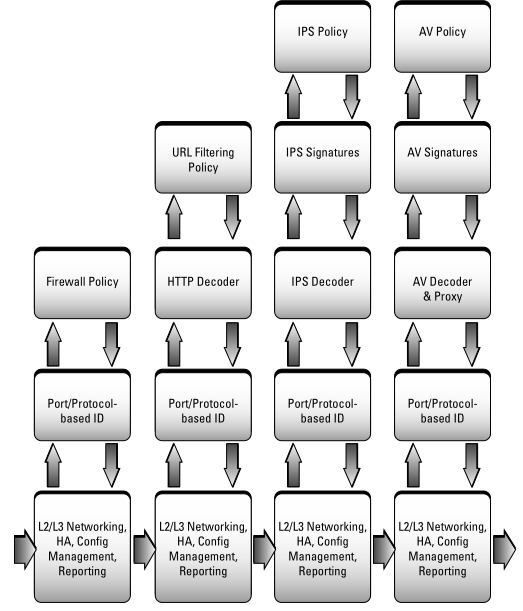
\includegraphics[width=8cm]{resources/architecture_tradisional_firewall.png}
	\caption{arsitektur proses tradisional firewall(\cite{miller2011next})}
	\label{fig:architecture_tradisional_firewall}
\end{figure}

Sebaliknya, \textit{new generation firewall} menggunakan \textit{single-pass architecture} untuk mengeliminasi pengecekan paket secara repetitif, mengurangi beban pada perangkat keras dan meminimalkan \textit{latency}, seperti yang dapat dilihat pada gambar berikut.

\begin{figure}[H]
	\centering
	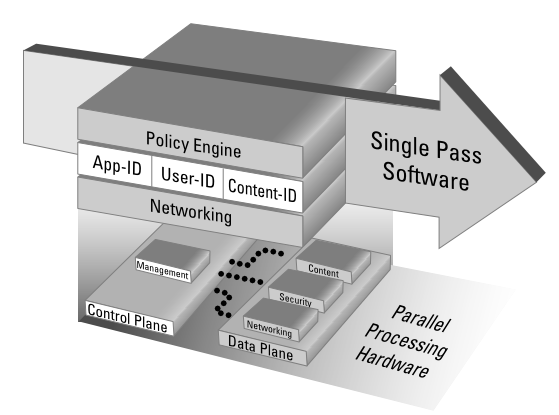
\includegraphics[width=0.7\textwidth]{resources/architecture_NGFW.png}
	\caption{Arsitektur proses \textit{new generation firewall}(\cite{miller2011next})}
	\label{fig:architecture_NGFW}
\end{figure}

\section{\textit{Deep Packet Inspection}}
\textit{Deep Packet Inspection} (DPI) adalah salah satu teknologi utama untuk mengidentifikasi dan mengotentikasi protokol dan aplikasi yang dibawa bersama IP (\cite{allot2007digging}). \textit{Standard packet inspection process} hanya mengekstrak informasi dasar dari suatu protokol seperti \textit{IP address} (tujuan, sumber) dan informasi koneksi \textit{low-level} lainnya, yang biasanya berada pada \textit{header} paket tersebut. Inspeksi ini tidak mendapatkan informasi yang cukup untuk dapat menyimpulkan apakah aplikasi tersebut aman atau tidak. 
\begin{figure}[H]
	\centering
	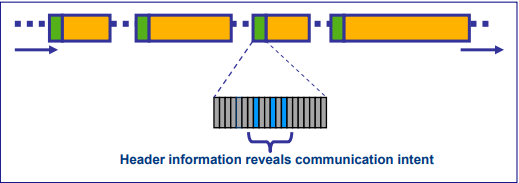
\includegraphics[width=0.8\textwidth]{resources/standard_inspection.png}
	\caption{\textit{Standard packet inspection} (\cite{allot2007digging})}
	\label{fig:standard_inspection}
\end{figure}
Sebaliknya, DPI menyediakan informasi tentang aplikasi tersebut. Hal ini dicapai dengan menganalisis konten pada \textit{header} paket dan \textit{payload} paket pada suatu transaksi paket. Oleh karena itu, DPI dapat menyediakan kemampuan untuk penganalisis penggunaan jaringan dan mengoptimasi kinerja jaringan. 

Komponen yang digunakan untuk memberi identitas pada aplikasi dan protokol disebut \textit{signature}. \textit{Signature} ini dapat juga diumpamakan seperti \textit{fingerprint} pada manusia, di mana tidak ada yang sama satu dengan yang lainnya. Oleh karena itu, \textit{signature} digunakan untuk mengidentifikasi aplikasi dan protokol. Signature pada aplikasi harus dicek secara berkala, karena signature tersebut dapat berubah seiring aplikasi \textit{update} atau revisi protokol.

Walaupun \textit{signature} tersebut dikembangkan dengan tujuan keunikan dan untuk mengidentifikasi suatu aplikasi atau protokol, ada kalanya \textit{signature} tersebut tidak robust. Terdapat istilah \textit{false positives} dan \textit{false negatives} karena \textit{signature} tersebut. \textit{False positives} merujuk pada keadaan salah mengelompokkan atau salah mengidentifikasi, seperti suatu aplikasi diidentifikasi sebagai sesuatu, namun sebenarnya bukan. \textit{False negatives} merujuk pada keadaan di mana suatu aplikasi atau protokol tidak ter-identifikasi secara konsisten sebagai sesuatu yang sama. Contohnya, beberapa aplikasi akan berperilaku berbeda apabila koneksi yang dilakukan melalui \textit{proxy} atau tidak. Salah satu cara untuk membuat \textit{signature} tersebut menjadi lebih \textit{robust} adalah dengan menggunakan beberapa pola kombinasi.

Ada beberapa metode analisis yang digunakan untuk mengidentifikasi dan mengelompokkan paket, yaitu:
\begin{itemize}
	\item Analisis berdasarkan port\\
	Analisis ini merupakan analisis yang paling mudah dan paling dikenal. Namun analisis ini tidak cukup untuk mengidentifikasi aplikasi sendirian, dikarenakan sudah banyak aplikasi yang memakai \textit{random port} atau menyamar sebagai aplikasi lain pada port tertentu.
	\item Analisis berdasarkan \textit{string match}\\
	Analisis ini akan mencari suatu string pada konten paket tersebut. Hal ini dilakukan karena banyak aplikasi yang menyertakan nama aplikasi tersebut pada protokolnya. 
	\item Analisis berdasarkan \textit{numerical properties}\\
	Analisis ini melibatkan perhitungan dan karakteristik numerik pada paket tersebut, seperti \textit{payload length}, banyaknya paket yang dikirim untuk respons transaksi tertentu, dan \textit{numerical offset} dari suatu \textit{string} dalam paket tersebut. Analisis ini juga tidak cukup berdiri sendiri untuk mengidentifikasi aplikasi.
	\item Analisis berdasarkan perilaku dan heuristik\\
	Analisis ini merujuk pada bagaimana biasanya protokol berperilaku dan beroperasi. Analisis heuristik pada umumnya berasal dari hasil statistik dari paket yang diamati.
\end{itemize}

\section{Malware}
\textit{Malicious software} menurut (\cite{idika2007survey}) memiliki banyak bentuk salah satunya adalah \textit{Malicious Code} (MC). Menurut (\cite{attackingmalcode}), \textit{malicious code} merupakan kode yang ditambahkan, diubah, atau dihilangkan dari sistem perangkat lunak untuk membahayakan atau mengubah fungsi yang diharapkan dapat dilakukan oleh sistem.

Virus merupakan program komputer yang memperbanyak diri dengan menyisipkan dirinya ke program lain. Program yang disisipi oleh virus menjadi terinfeksi disebut inang. Hal ini yang membedakan virus dengan malware lain, untuk melakukan fungsinya virus memerlukan inang (\cite{attackingmalcode}).

Worm merupakan program komputer yang memperbanyak diri dirinya dengan menjalankan kode worm yang menjadi sebuah program tersendiri. Bagian yang membedakan worm dan virus, worm tidak memerlukan inang untuk melakukan fungsinya. Selain itu, virus dan worm juga berbeda pada cara penyebarannya. Pada umumnya, virus berusaha untuk menyebar melalui file atau program pada satu komputer. Sedangkan worm berusaha untuk menginfeksi sebanyak mungkin komputer melalui jaringan (\cite{attackingmalcode}).

\textit{Trojan horse} merupakan \textit{malicious code} yang tambahkan oleh desainer dalam sebuah aplikasi atau sistem. Aplikasi tersebut menjalankan fungsinya, namun melakukan aktifitas \textit{malicious} seperti merekam kegiatan pengguna dan mengirimkannya ke pembuatnya. \textit{Trojan horse} pada umumnya berkaitan dengan mengakses dan mengirimkan informasi tanpa otorisasi dari pengguna. \textit{Trojan horse} dapat dikategorikan sebagai \textit{spyware}. 

\section{Infeksi Malware}
Perilaku menginfeksi malware berbeda untuk masing-masing jenis malware. Klasifikasi ini dilakukan dari sudut pandang bagaimana malware dapat dideteksi dan bagaimana malware menyembunyikan diri. Dalam penelitian ini dibahas tiga jenis infeksi malware, yakni: virus, worm, dan bot sebagai dasar pembahasan analisis yang akan dilakukan pada bab III.

\subsection{Infeksi Virus}

Infeksi oleh virus dilakukan dengan cara menyisipkan kode ke executable lain (host). Bagian penting dari infeksi oleh malware kategori virus berada pada bagaimana virus menyembunyikan diri pada executable host. Beberapa cara menyembunyikan diri dari (\cite{6620049}) dan (\cite{alsamer2016}) yakni: \textit{obfuscation}, enkripsi, \textit{oligomorphic}, \textit{polymorphic}, \textit{metamorphic}.

Teknik \textit{obfuscation} dilakukan dengan cara menambahkan perintah \textit{garbage} kedalam kode. Perintah \textit{garbage} dapat berupa perintah seperti nop pada assembly atau pun jump yang membuat kode virus terpotong-potong sehingga membuat \textit{signature} menjadi lebih sulit didapatkan.

Selain itu beberapa virus menggunakan teknik enkripsi untuk mengodekan dirinya. Virus dengan jenis ini memiliki algoritma cipher, kunci, dan kode \textit{malicious} yang terenkripsi. Teknik ini menjadikan virus dengan jenis ini kompleks.

\textit{Oligomorphic} merupakan teknik menyembunyikan diri dengan teknik enkripsi tetapi menggunakan algoritma cipher yang berubah dalam jangka waktu tertentu. Virus dengan jenis ini akan memiliki beberapa algoritma cipher yang dapat digunakan, di mana algoritma cipher akan berulang pada saat tertentu.

Sedangkan pada teknik \textit{polymorphic}, virus memiliki algoritma cipher yang tak terhingga banyaknya. Virus dengan jenis ini memiliki algoritma untuk membuat algoritma ciphernya secara acak. Sehingga untuk setiap infeksi, virus ini memiliki algoritma cipher baru dan kunci cipher baru.

Teknik \textit{metaphoric} merupakan teknik virus yang dapat menyembunyikan dirinya dalam bentuk lain yang tidak memiliki kemiripan dengan kode asalnya. Virus dengan jenis ini tidak memiliki algoritma cipher, namun untuk setiap infeksi kode dirinya berubah.

\subsection{Infeksi Worm}

Worm pada (\cite{alsamer2016}) disebut sebagai \textit{subclass} dari virus yang dapat hidup tersendiri. Worm memiliki karakteristik untuk dapat menyebarkan dirinya melalui jaringan dengan melakukan eksploit terhadap \textit{vulnerability} atau kesalahan pengaturan pada \textit{service} yang digunakan secara umum. Worm dapat dikategorikan menjadi dua kategori yakni: \textit{scan-based worm} dan \textit{topology-based worm}.

\textit{Scan-based worm} merupakan mencoba melakukan pemindaian lingkungan untuk dapat menginfeksi. Teknik pemindaian dapat berbentuk \textit{random scanning} atau \textit{localized scanning}. \textit{Random scanning} dilakukan dengan menemukan host secara acak yang dapat di-infeksi. Teknik untuk menemukan secara acak dapat menggunakan \textit{random number generator}, \textit{list} atau host yang dapat diakses melalui \textit{routing}. \textit{Localized-scanning} dilakukan dengan cara menemukan host dalam linkungan yang tertentu untuk di-infeksi. \textit{Localized} yang dimaksud dapat berbentuk grup lokal yang memang ditargetkan oleh penyerang, atau jangkauan IP tertentu, atau secara melakukan pemindaian sekuensial dari IP. \textit{Localized-scanning} dapat memperkecil waktu untuk penyebaran dibandingkan dengan \textit{random scanning} karena malware memiliki pengetahuan tambahan dibanding \textit{random-scanning}.

\textit{Topology-based worm} melakukan infeksi dengan cara menemukan tetangga dari topologi yang dimiliki host. Jenis worm ini memiliki peluang yang berbeda untuk setiap usaha melakukan infeksinya. Penyebarannya memiliki karakteristik khusus, yakni memiliki \textit{user interference}. Peluang terjadinya \textit{user interference} berbeda-beda akibat beberapa faktor yang dimiliki oleh korban. Salah satu contoh \textit{user interference} yang dimanfaatkan oleh worm kategori ini berupa surel. Surel digunakan oleh worm untuk mengirimkan salinan nya misal dalam bentuk \textit{attachment}. Sehingga peluang penyebarannya akan bergantung pada faktor berapa sering korban membuka surel dan membuka \textit{attachment}.

\subsection{Infeksi Bot}

Hal yang perlu diperhatikan pada infeksi bot berada pada fase dan komponen malware ini. Menurut (\cite{alsamer2016}) fase pada malware kelas ini adalah: \textit{infection}, \textit{spreading}, \textit{rallying}, dan \textit{elusion}.

Pada fase \textit{infection} malware pada umumnya dijalankan oleh penyerang pada sebuah host. Ketika host sudah terinfeksi, maka malware akan melanjutkan ke fasa selanjutnya, yaitu \textit{spreading}. Pada fasa \textit{spreading}, bot akan melakukan infeksi dapat berupa aktif maupun pasif (\cite{alsamer2016}). Penyebaran secara aktif dilakukan dengan cara \textit{scanning} seperti yang dilakukan oleh worm. Sedangkan penyebaran secara pasif dilakukan dengan mengandalkan \textit{user inferference} yakni teknik seperti teknik \textit{topology} yang digunakan pada worm.

Fasa \textit{rallying}, bot akan melakukan kontak dengan \textit{control server} untuk mendapatkan perintah. Perintah dapat dikategorikan menjadi: pengintaian \textit{traffic}, \textit{denial of service}, \textit{compute power}, \textit{spam}, dan menjadi saluran penyebaran malware. Untuk melakukan kontak dengan \textit{control server}, malware dapat menggunakan IP, nama domain, atau pun menggunakan suatu algoritma yang dimiliki malware (\cite{alsamer2016}). Bagian ini merupakan bagian paling penting dalam malware kelas ini, karena bot tanpa adanya komunikasi dengan \textit{control server} tidak memiliki tujuan (\cite{alsamer2016}). Selain itu bagian ini merupakan bagian yang paling mudah untuk dijadikan \textit{signature}, misalnya dengan menemukan IP atau nama domain tertentu. Sehingga beberapa malware menggunakan teknik seperti \textit{IP flux} atau \textit{DNS flux}. Selain itu koneksi yang dilakukan dengan \textit{control server} dapat menggunakan jaringan anonim, enkripsi, atau \textit{tunneling}.

Fase ini juga bersamaan dengan fasa \textit{elusion}. Fase \textit{elusion}, bot harus dapat menyembunyikan dirinya seperti mekanisme seperti \textit{polymorphism} yang dimiliki oleh kategori virus sehingga mempersulit \textit{signature} dari bot untuk dikenali. 

\section{Malware Detection}

Pada (\cite{idika2007survey}) teknik untuk mendeteksi malware dibedakan menjadi dua, yakni: \textit{signature-
based} dan \textit{anomaly-based}. Terdapat bentuk khusus \textit{anomaly-based} yakni \textit{specification-based}. Setiap teknik memiliki jenis pendekatan \textit{static}, \textit{dynamic}, dan \textit{hybrid}.

\subsection{Anomaly-based Detection}

Pada (\cite{idika2007survey}) dijelaskan, \textit{anomaly-based detection} memiliki dua fase, yakni fase \textit{training}, dan fase deteksi. Pendeteksian jenis ini memiliki kelebihan, yakni dapat mendeteksi serangan yang sebelumnya belum dikenali. Namun, deteksi jenis ini memiliki tingkat kesalahan pendeteksian yang tinggi. \textit{Anomaly based-detection} melakukan pendeteksian dengan cara membuat pendekatan perilaku yang \textit{valid} dilakukan oleh sebuah sistem.

\begin{figure}[H]
	\centering
	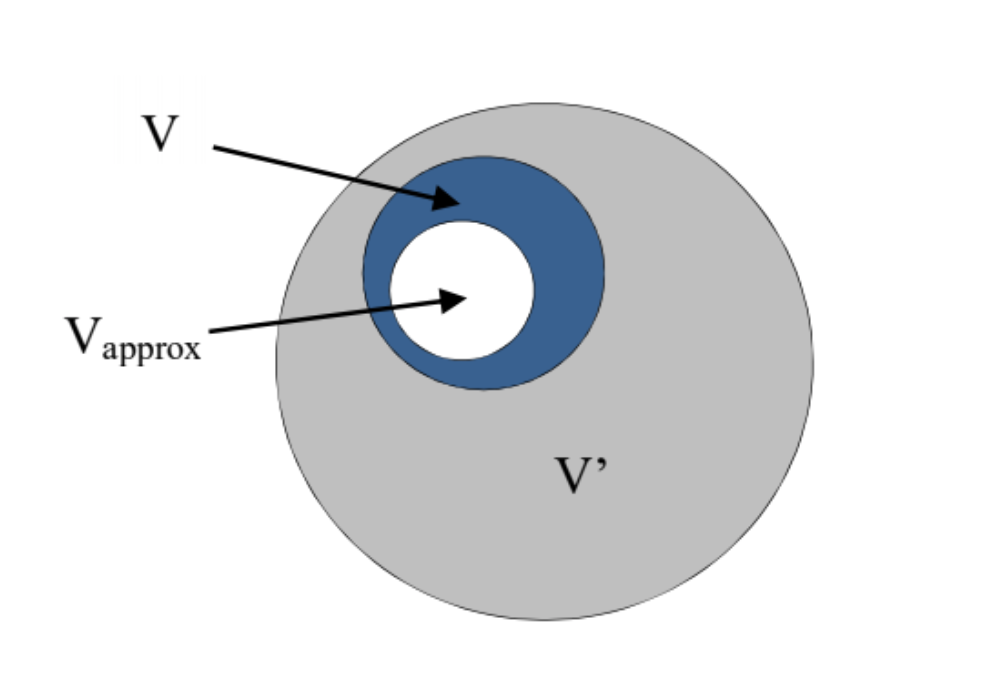
\includegraphics[width=220px]{resources/anomaly_illustration.png}
	\caption{Ilustrasi karakterisasi perilaku pada \textit{anomaly-based detection} (\cite{idika2007survey})}
	\label{fig:anomaly_illust}
\end{figure}

Gambar \ref{fig:anomaly_illust} menggambarkan bagaimana \textit{anomaly-based detection} mengkarakterisasi perilaku sistem. V merupakan himpunan perilaku yang tidak bertentangan dengan \textit{requirement}. V’ merupakan himpunan perilaku yang yang tidak valid. Vapprox merupakan hasil pendekatan yang dilakukan oleh \textit{anomaly-based detection}.

\subsection{Signature-based Detection}
\textit{Signature-based detection} dalam (\cite{idika2007survey}) merupakan teknik yang menggunakan \textit{malicious-model} untuk mendeteksi malware. Kumpulan dari \textit{malicious-model} (signature) menjadi \textit{knowledge base} dari sistem pendeteksi jenis ini. Sehingga pada Gambar \ref{fig:signature_illust}, diilustrasikan bahwa S (kumpulan \textit{signature}) merupakan himpunan bagian dari U yang merupakan seluruh \textit{signature} dari perilaku \textit{malicious}. Karena keterbatasan media penyimpanan, S akan sangat kecil jika dibandingkan dengan U yang sangat besar.

\begin{figure}[H]
	\centering
	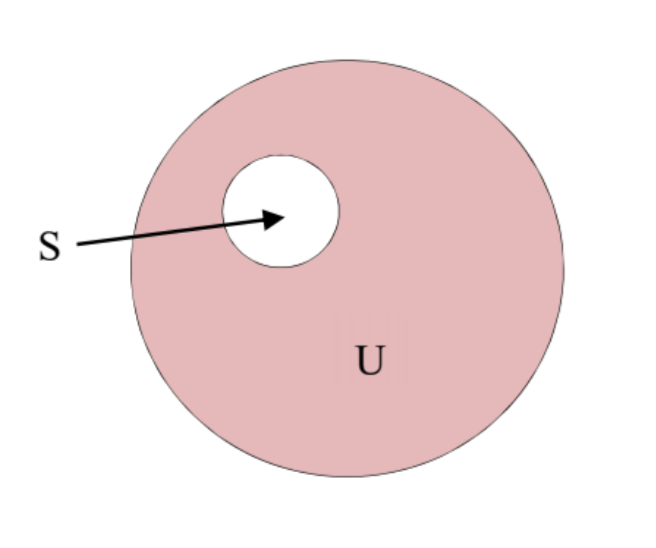
\includegraphics[width=190px]{resources/signature_illustration.png}
	\caption{Ilustrasi himpunan \textit{signature} terhadap seluruh \textit{malicious} signature (\cite{idika2007survey})}
	\label{fig:signature_illust}
\end{figure}

\section{Iptables}
Pada (\cite{rash2007linux}) dijelaskan, iptables firewall dikembangkan oleh \textit{NetFilter Project} \textit{(http://www.netfilter.org)}, dan sudah menjadi bagian dari kernel linux sejak Januari 2001.  Pada masa ini, iptables sudah banyak digunakan pada firewall komersial. Hal ini dikarenakan Iptables mempunyai protokol \textit{state tracking} yang komprehensif, \textit{packet application layer inspection}, pembatasan kecepatan, dan mekanisme untuk mengatur \textit{filtering policy} yang mumpuni. 
Istilah Iptables dan Netfilter cukup membingungkan untuk banyak orang pada komunitas Linux. Menurut (\cite{purdy2004linux}) Netfilter adalah bagian dari kernel Linux yang berfungsi untuk memproses paket dari jaringan. Sementara itu,  iptables adalah perintah untuk mengatur \textit{Netfilter} yang dapat digunakan pada \textit{user-space}. 

Suatu iptables \textit{policy} dibuat dari suatu set aturan yang akan mengatur rute dari suatu paket. Setiap set aturan tersebut diaplikasikan pada \textit{chain} di dalam satu tabel tersendiri. Tabel tersebut dikelompokkan berdasarkan fungsinya, yaitu filter, \textit{Network address translation} (NAT) dan \textit{packet mangling}. Fungsi dari filter adalah untuk mengatur keluar masuknya paket yang masuk ke komputer tersebut. Fungsi NAT digunakan dengan \textit{connection tracking} untuk melakukan \textit{Network Address Translation} (NAT). Dan yang terakhir, fungsi \textit{packet mangling} digunakan untuk manipulasi paket.

\subsection{Alur pemrosesan paket}
Setiap table memiliki \textit{chain} (urutan) pemrosesannya masing-masing. Alur pemrosesan dasar tersebut dapat dilihat pada gambar-gambar dibawah ini.
\begin{figure}[H]
	\centering
	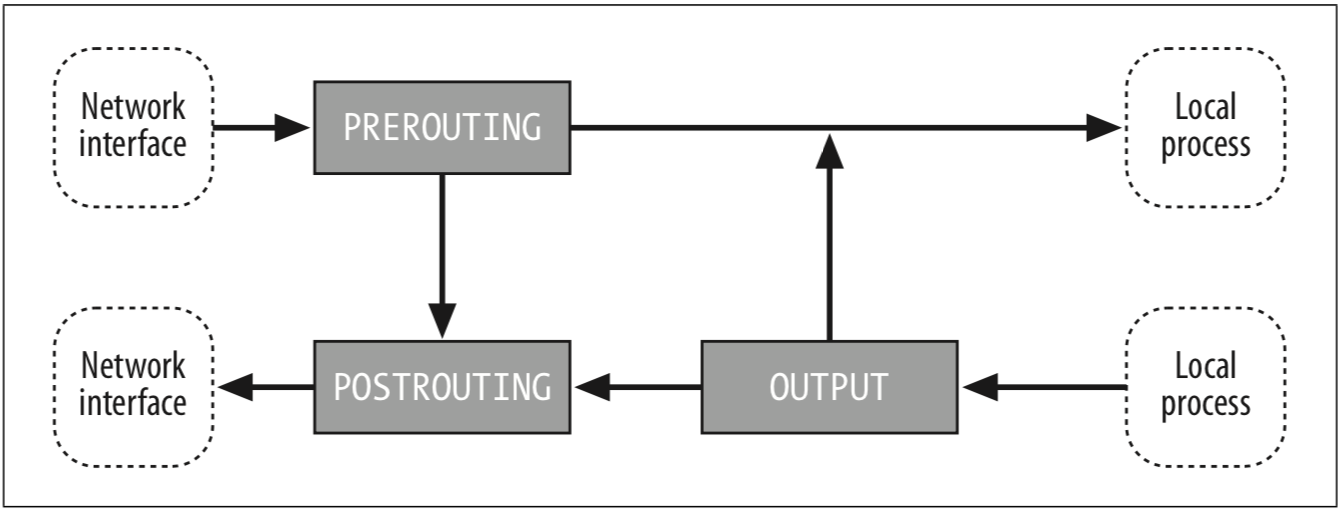
\includegraphics[width=\textwidth]{resources/nat_table.png}
	\caption{Alur pemrosesan paket dan \textit{hook} yang digunakan pada tabel \textit{NAT}. (\cite{purdy2004linux})}
	\label{fig:packetflow_NAT}
\end{figure}

\begin{figure}[H]
	\centering
	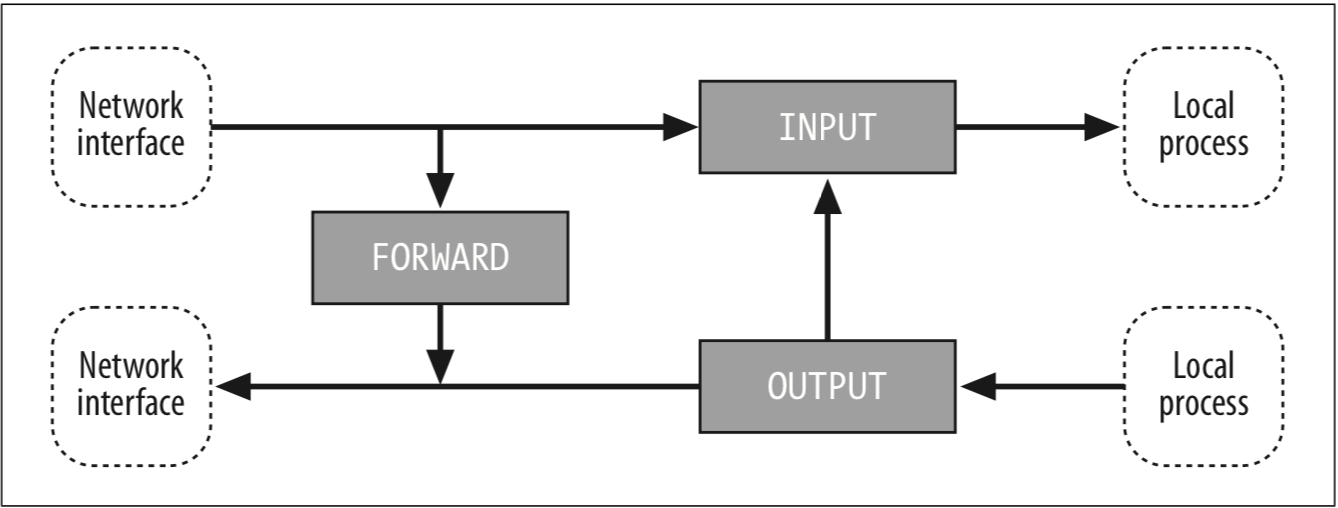
\includegraphics[width=\textwidth]{resources/filter_table.png}
	\caption{Alur pemrosesan paket dan \textit{hook} yang digunakan pada tabel \textit{filter}.(\cite{purdy2004linux})}
	\label{fig:packetflow_filter}
\end{figure}

\begin{figure}[H]
	\centering
	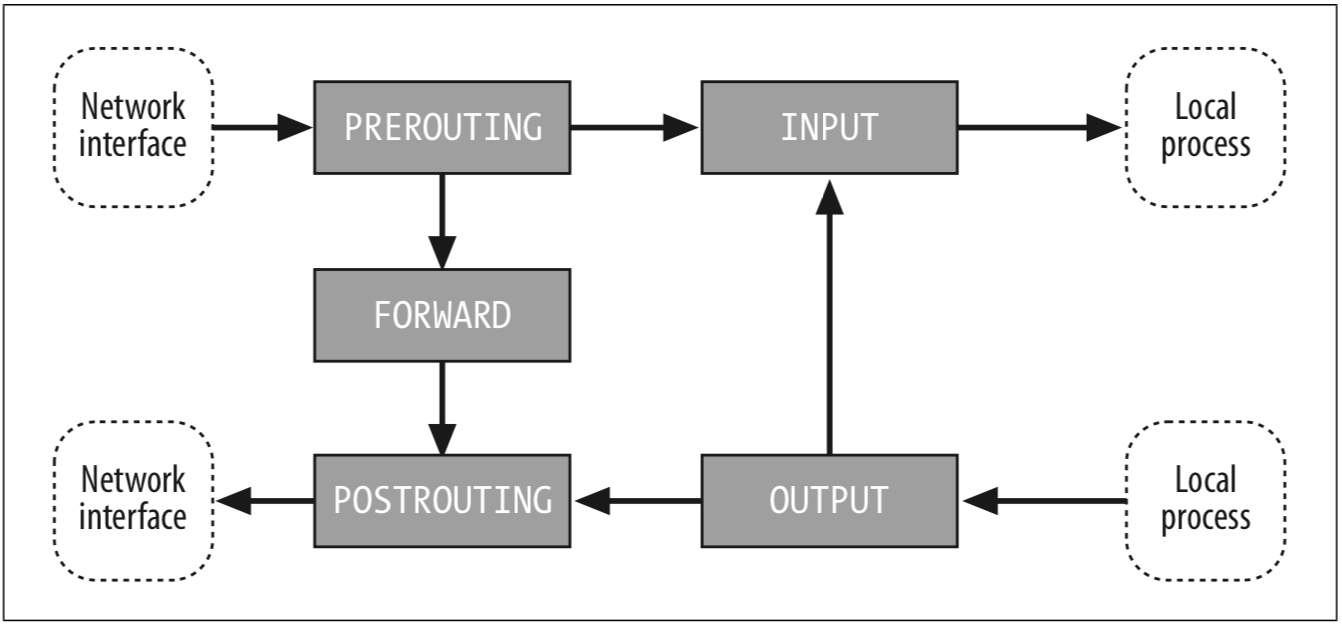
\includegraphics[width=\textwidth]{resources/mangling_table.png}
	\caption{Alur pemrosesan paket dan \textit{hook} yang digunakan pada tabel \textit{mangling}.(\cite{purdy2004linux})}
	\label{fig:packetflow_mangling}
\end{figure}

Poin-poin yang terdapat pada gambar-gambar di atas adalah \textit{hook} poin yang memiliki fungsi-fungsi tersendiri.\textit{Netfilter} memiliki 5 poin (\textit{hook}) di dalam alur pemrosesan paket, yaitu : \textit{PREROUTING}, \textit{INPUT}, \textit{FORWARD}, \textit{POSTROUTING}, \textit{POSTROUTING}, dan  \textit{OUTPUT}. 
Poin \textit{PREROUTING} akan memproses paket yang baru datang dari \textit{network interface} (setelah melalui proses pengecekan \textit{checksum}).
Poin \textit{INPUT} akan memproses paket yang akan dilanjutkan ke proses lokal.
Poin \textit{FORWARD} akan memproses paket yang keluar masuk melalui \textit{gateway} komputer.
Poin \textit{POSTROUTING} akan memproses paket yang akan meninggalkan \textit{network interface}.
Poin \textit{OUTPUT} akan memproses paket yang baru saja melewati proses lokal.


Built-in chain yang paling umum dipakai untuk membuat firewall adalah INPUT, OUTPUT dan FORWARD, yang berada pada \textit{filter table}. INPUT chain akan dijalankan satu-persatu oleh paket yang seharusnya memasuki sistem lokal, sementara OUTPUT chain akan dijalankan satu persatu oleh paket yang berasal dari sistem lokal tersebut. Sedangkan FORWARD chain, oleh paket yang melewati sistem tersebut yang bukan ditujukan untuk sistem lokal. Untuk lebih jelasnya, dapat dilihat pada gambar dibawah ini (\ref{fig:iptables_packet_flow}). 
\begin{figure}[H]
	\centering
	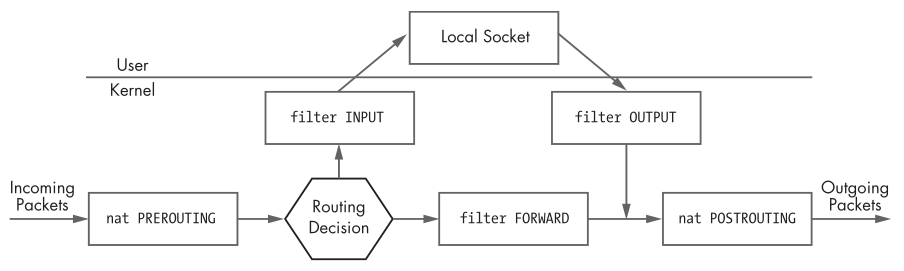
\includegraphics[width=\textwidth]{resources/iptables_packet_flow.png}
	\caption{Contoh alur pemrosesan paket yang melewati tabel NAT dan tabel filter.(\cite{rash2007linux})}
	\label{fig:iptables_packet_flow}
\end{figure}

Paket yang melewati \textit{chain} akan terkena aturan sesuai dengan urutannya. Apabila paket tersebut tidak sesuai kriteria, maka paket akan bergerak ke aturan selanjutnya. Jika paket tersebut tidak memenuhi kriteria sampai aturan yang paling akhir, maka paket tersebut akan diperlakukan sesuai dengan \textit{chain\textquotesingle s policy}. 
Berdasarkan Gambar , urutan alur paket yang melewati \textit{tables} dan \textit{chains} dapat dilihat pada tabel-tabel berikut.

\begin{table}[H]
	\caption{Alur paket yang melewati network interface ke network interface lainnya (forwarding) (\cite{purdy2004linux})}
	\label{table:network_to_network}
	\centering
	\begin{tabular}{ll}
		\hline
		\rowcolor[HTML]{C0C0C0} 
		table  & chain       \\ \hline
		mangle & PREROUTING  \\
		nat    & PREROUTING  \\
		mangle & FORWARD     \\
		filter & FORWARD     \\
		mangle & POSTROUTING \\
		nat    & POSTROUTING \\ \hline
	\end{tabular}
\end{table}

\begin{table}[H]
	\caption{Alur paket yang melewati \textit{network interface} ke proses lokal (input)(\cite{purdy2004linux})}
	\label{table:network_to_local}
	\centering
	\begin{tabular}{ll}
		\hline
		\rowcolor[HTML]{C0C0C0} 
		table  & chain      \\ \hline
		mangle & PREROUTING \\
		nat    & PREROUTING \\
		mangle & INPUT      \\
		filter & INPUT      \\ \hline
	\end{tabular}	
\end{table}

\begin{table}[H]
	\caption{Alur paket yang datang dari proses lokal ke \textit{network interface} (output) (\cite{purdy2004linux})}
	\label{table:local_to_network}
	\centering
	\begin{tabular}{ll}
		\hline
		\rowcolor[HTML]{C0C0C0} 
		table  & chain       \\ \hline
		mangle & OUTPUT      \\
		nat    & OUTPUT      \\
		filter & OUTPUT      \\
		mangle & POSTROUTING \\
		nat    & POSTROUTING \\ \hline
	\end{tabular}
\end{table}

\begin{table}[H]
	\caption{Alur paket yang datang dari proses lokal ke proses lokal lainnya (local)(\cite{purdy2004linux})}
	\label{table:local_to_local}
	\centering
	\begin{tabular}{ll}
		\hline
		\rowcolor[HTML]{C0C0C0} 
		table  & chain  \\ \hline
		mangle & OUTPUT \\
		nat    & OUTPUT \\
		filter & OUTPUT \\
		filter & INPUT  \\
		mangle & INPUT  \\ \hline
	\end{tabular}
\end{table}
\subsection{Matches dan Target}
Setiap Iptables mempunyai satu set aturan berisikan syarat (\textit{matches}) dan target. Syarat dari aturan tersebut akan menentukan paket mana saja yang akan terkena aturan tersebut, sementara target akan menentukan apa yang akan dilakukan oleh paket yang memenuhi syarat tersebut. Apabila tidak ada syarat (\textit{match criteria}) maka semua paket dianggap memenuhi syarat. Sebaliknya, apabila tidak ada target, maka paket tidak akan diproses. Syarat yang dapat digunakan antara lain adalah IP (\textit{Internet Protocol}) dan \textit{MAC addresses}.
Netfilter memiliki beberapa \textit{built-in target}, yaitu: \textit{ACCEPT}, \textit{DROP}, \textit{QUEUE}, dan \textit{RETURN}. 
\textit{ACCEPT} akan mengizinkan paket untuk menuju proses selanjutnya,
\textit{DROP} akan menghentikan proses paket sepenuhnya,
\textit{QUEUE}akan mengirimkan paket ke \textit{userspace}, dan 
\textit{RETURN}akan menghentikan proses pada \textit{user-defined chain} dan melanjutkan proses ke \textit{chain} sebelum user-defined chain dipanggil.